\subsection{Frozen-coefficient diagnostic}

    A controlled experiment holds the reference Neural SDE coefficients fixed
    and simulates each of the 42 observed transitions from its observed starting
    state. Each setting uses 5000 paths and simulation seeds 8, 9, and 10.
    Dividing an observation interval into 1, 16, or 64 Euler--Maruyama steps
    changes only the forward approximation, not the fitted coefficients.
    Table~\ref{tab:frozen-transitions} shows that the favorable one-step
    coverage does not persist under refinement. The distinction between
    discretization error and stochastic variability is fundamental to the
    numerical interpretation of an SDE \citep{higham2001algorithmic}.

% Generated by scripts/build_iteration_tables.py; do not edit manually.
\begin{table}[htbp]
\centering
\caption{Frozen reference coefficients: conditional simulations averaged over three seeds.}
\label{tab:frozen-transitions}
\begingroup\small\setlength{\tabcolsep}{4pt}
\begin{tabular}{rrrr}
\toprule
Substeps & RMSE & Coverage & RMS mean shift \\
\midrule
1 & 1.2794 & 0.9365 & 0.0153 \\
16 & 1.5143 & 0.5159 & 0.6735 \\
64 & 1.5308 & 0.5079 & 0.6838 \\
\bottomrule
\end{tabular}
\endgroup
\end{table}
\begin{table}[htbp]
\centering
\caption{Controlled candidates: nominal interval level 0.90. Held-out summaries reuse observations across cutoffs.}
\label{tab:rev07-forecast}
\begingroup\small\setlength{\tabcolsep}{4pt}
\begin{tabular}{lrrrr}
\toprule
Candidate & Full-data coverage & Held-out coverage & RMSE & Width \\
\midrule
Wide Euler & 0.6071 & 0.0694 & 3.1357 & 1.4974 \\
Wide moments & 0.8929 & 0.4120 & 2.1000 & 2.5063 \\
Small Euler & 0.7579 & 0.3380 & 1.5335 & 1.4451 \\
Small moments & 0.9444 & 0.4583 & 1.6204 & 2.2985 \\
Small moments + L2 & 0.9722 & 0.4306 & 1.9365 & 2.5716 \\
Logistic + observation noise & 0.9048 & 0.5000 & 2.6531 & 3.3983 \\
\bottomrule
\end{tabular}
\endgroup
\end{table}


    At the observed states, the dimensionless quantity
    \(\partial_z\mu_\theta(\tau_i,z_i^{[j]})\Delta\tau_i\) ranges from
    \(-3.656\) to \(0.037\). Six transitions have this quantity below \(-2\),
    outside the explicit-Euler stability interval for a frozen negative linear
    drift. This local linearization gives a concrete mechanism for disagreement
    between a coarse transition and refined dynamics. It is not a global
    nonlinear stability theorem or a complete explanation of forecast error.

\subsection{Controlled transition and architecture comparisons}

    Five neural candidates compare two coefficient architectures (32 units in
    two hidden layers, or 8 units in one hidden layer), one-step versus
    16-substep transition objectives, and a stronger weight decay for the small
    refined candidate. The respective parameter counts are 2370 and 66.
    Standard weight decay is \(10^{-4}\); the stronger setting is \(10^{-2}\).
    All use 1000 Adam epochs, learning rate \(0.005\), and gradient clipping at
    10. Each candidate is initialized independently with training seeds 7 and
    17. These matched-initialization controls differ from the original reference
    checkpoint, whose random-number stream followed Neural ODE training.

    The refined transition uses a Gaussian assumed-density approximation
    \citep{sarkka2019applied}. For a Gaussian state with mean \(m\) and variance
    \(v\), let \(x_q=m+\sqrt{v}\,\xi_q\), where
    \(\xi_q\in\{-\sqrt{3},0,\sqrt{3}\}\) and
    \(w_q\in\{1/6,2/3,1/6\}\). For an internal step \(h\), define
    \[
        a_q=x_q+h\mu_\theta(\tau,x_q),\qquad
        m_+=\sum_q w_q a_q,
    \]
    \[
        v_+=\sum_q w_q(a_q-m_+)^2
            +h\sum_q w_q\sigma_\phi(\tau,x_q)^2.
    \]
    These expressions follow from total expectation and total variance for an
    Euler step. Projecting back to a Gaussian after each substep introduces
    closure error for nonlinear coefficients. Refinement does not make this
    transition density exact. The original variance floor is added once at
    the end of the observation interval. Analytic-moment and gradient tests
    validate the implementation; Monte Carlo checks assess the approximation
    for the fitted candidate.

\subsection{Time-respecting forecasting results}

    Separate fits train through times 108, 120, and 132 and forecast all
    remaining observations. Response and time normalization use training rows
    only. Future normalized times retain the training origin and may exceed
    one. A free forecast conditions on the last training observation without
    restarting from later test observations. The conditioning row is excluded
    from coverage. Each neural forecast uses 2000 paths, simulation seeds 8,
    9, and 10, and maximum normalized integration step \(0.001\).

    Table~\ref{tab:rev07-forecast} and Figure~\ref{fig:rev07-calibration} show
    that improved in-sample consistency does not establish forecast calibration.
    The compact refined model has approximately 94.4 percent full-data coverage
    but only 45.8 percent held-out coverage. Stronger regularization does not
    resolve the failure. The logistic comparator adds independent Gaussian
    observation error, estimated on training residuals, but also undercovers.
    It changes both the dynamics family and the observation model and therefore
    does not isolate observation noise as the cause.

    The three cutoffs give 36 overlapping forecast entries involving only
    15 distinct scalar observations. Averages over simulation and training
    seeds are descriptive; these are not 36 independent validation observations.
    No binomial confidence interval or definitive calibration claim follows.
    REV-07 remains open, and none of the candidates replaces the reference
    Neural SDE. The following section addresses the separate omission of an
    explicit observation model and parameter uncertainty.

\begin{figure}[htbp]
    \centering
    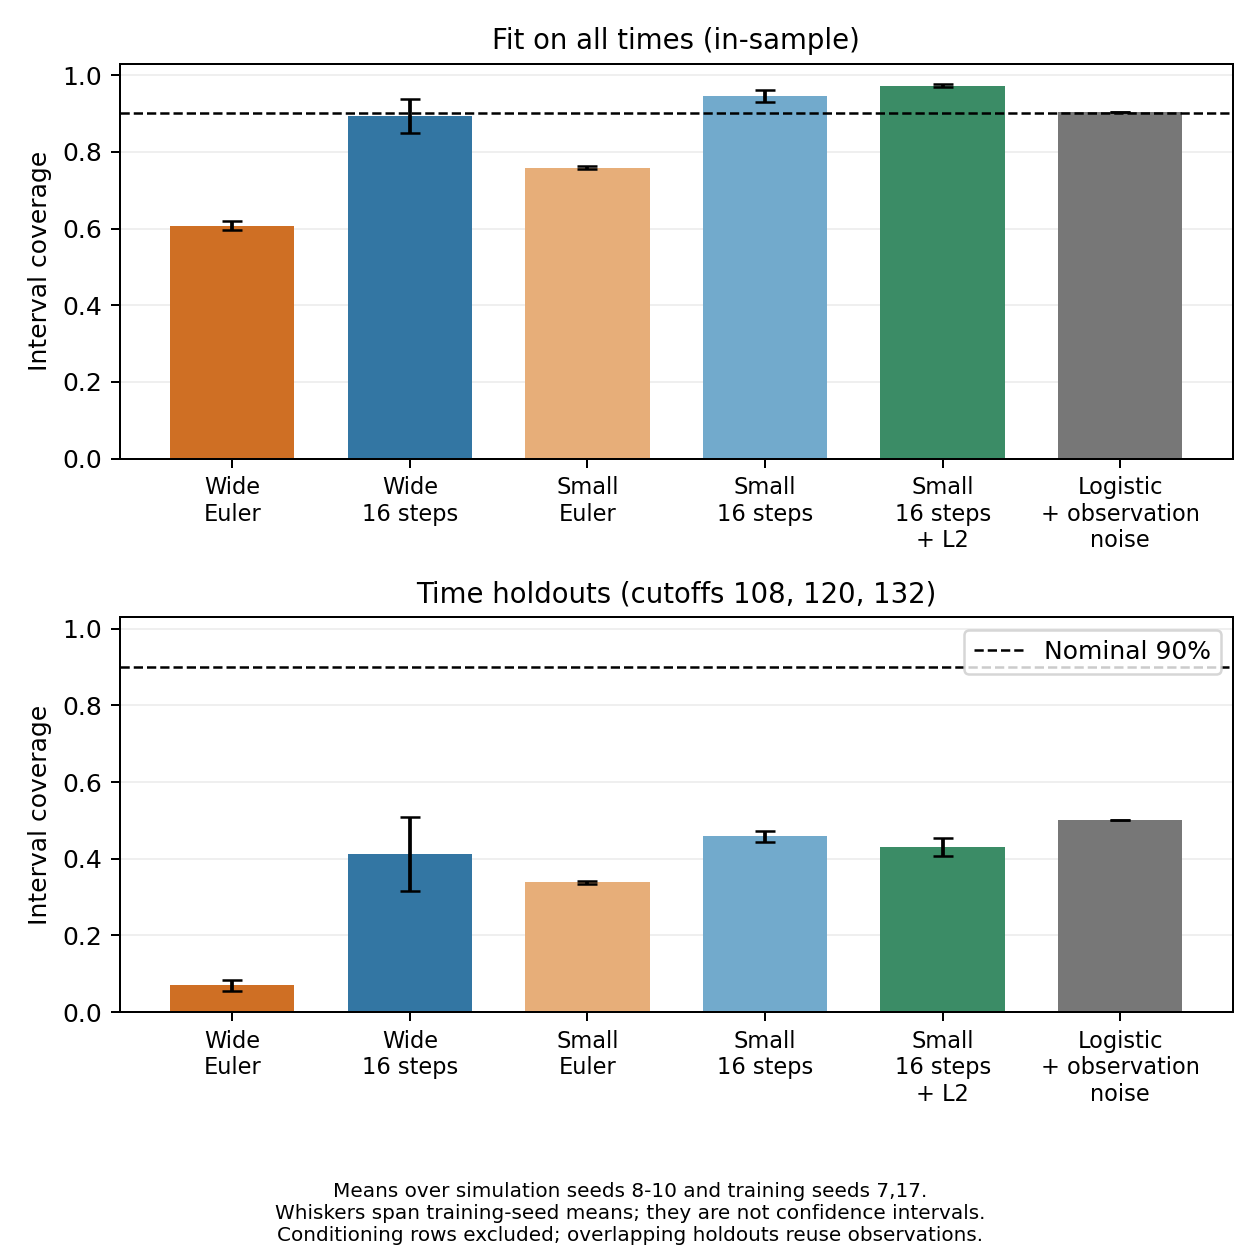
\includegraphics[width=\textwidth]{../results/rev07/calibration_summary.png}
    \caption{Coverage for the controlled candidates. All conditioning rows are
    excluded. Whiskers span training-seed averages, rather than confidence
    intervals. Overlapping forecast splits reuse observations.}
    \label{fig:rev07-calibration}
\end{figure}
